\problem{3: Network Coding}{4}
Network coding is a network paradigm where intermediate nodes in the network can compute functions on the incoming packets and send new packets on their output links. With this simple shift in the networking paradigm, Network coding promises to offer benefits along several dimensions such as throughput, security and resilience to link failures and packet losses.\\
The  benefit of network coding are often illustrated with the classic “Butterfly network” example shown in the figure below where S  is  the source and all the links have the same capacity. The goal is to maximize the receiving rate at the two receivers R1 and R2  in a multicast session. Without network coding, the optimal throughput of 1.5 packets/channel use can be achieved, while, with  network  coding,  if peer X  is able  to code  its input messages a and b into a+b, an effective end-to-end throughput of 2 packets/channel use can be achieved instead.\\


\begin{center}

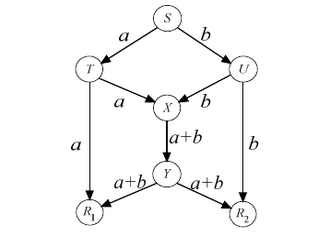
\includegraphics[scale=1]{./images/butterfly.png}

\end{center}

We ask you to emulate the butterfly topology in the picture in Mininet and deploy a P4 program on switch X that xor${s}$ packets' payloads.\\~\\~\\

\subproblem{Submission} This is an assignment for you to go wild with P4 and other tools you may have learned throughout this course (e.g., Mininet). Therefore, we are very open about the content of your submission. At the best, we would expect you to be able to implement this simple network coding function in P4, emulate the above topology with Mininet and showcase this function works at the end-hosts (for example, decoding by using a software library for network coding).

